@ -1,291 +1,300 @@
\chapter{Caso de estudio IMU y PID}
\label{ch:especifico3}

\section{Caso de estudio 2 - IMU}

Como caso de estudio de implementación se desarrolló también la simulación de una Unidad de medición inercial, IMU por sus siglas en Ingles, se siguió el uso del modelo que se presenta en \cite{mathworks2024imu}. Este ejemplo muestra cómo generar y fusionar datos de sensores IMU usando MATLAB Simulink. Permitiendo modelar con precisión el comportamiento de un acelerómetro, un giroscopio y un magnetómetro, además de poder fusionar sus salidas para calcular la orientación.

Una IMU es un grupo de sensores que incluye un acelerómetro para medir aceleración y un giroscopio para medir velocidad angular. Frecuentemente, también se incluye un magnetómetro para medir el campo magnético de la Tierra. Cada uno de estos tres sensores produce una medición de tres ejes, constituyendo una medición de 9 ejes en total. Ademas de esto un Sistema de Referencia de Actitud y Rumbo (AHRS, por sus siglas en inglés) toma las lecturas de sensores de 9 ejes y calcula la orientación del dispositivo. Esta orientación se da en relación con el marco NED, donde N es la dirección del Norte Magnético. El bloque AHRS en Simulink logra esto usando una estructura de filtro de Kalman indirecto \cite{mathworks2024imu}.

\subsection{Implementación en MATLAB Simulink}

\begin{figure}[h!]
    \centering
    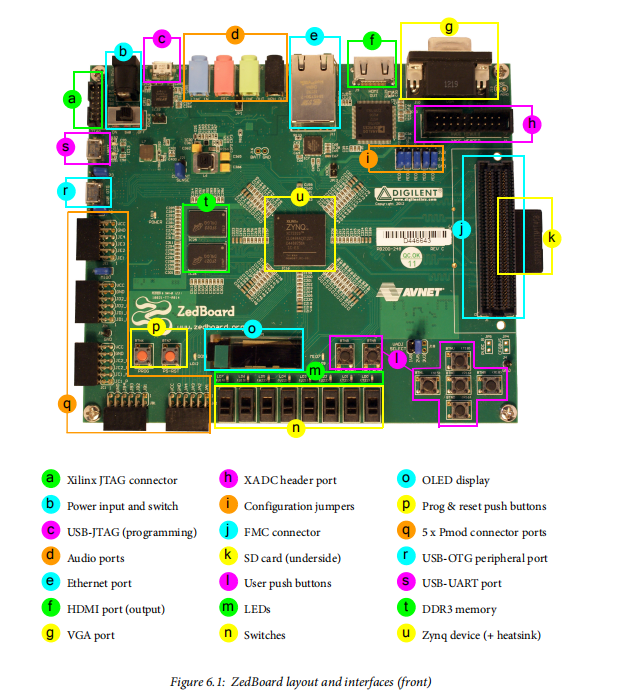
\includegraphics[width=0.8\textwidth]{fig/especifico_2/154140ZedBoard.png}
    \caption{Diagrama completo del caso de estudio 2 - IMU \cite{mathworks2024imu}}
    \label{fig:caso_de_estudio_2_IMU}
\end{figure}


Como se puede observar en la Figura \ref{fig:caso_de_estudio_2_IMU}, este es el caso de estudio que se propone en \cite{mathworks2024imu}, a este caso de estudio se le deben de realizar unas modificaciones de acuerdo al funcionamiento deseado que se tiene para este caso de estudio, siempre generando datos en el ámbito de simulación en MATLAB para luego contrastar los mismos con los datos obtenidos en la ejecución del modelo en la tarjeta de desarrollo seleccionada.

\subsection{Bloques utilizados para la implementación}

Los bloques utilizados se obtienen en la librería de bloques de MATLAB Simulink. A continuación se muestran los bloques requeridos, asi como la configuración de los mismos para la correcta operación del modelo. La implementación del sistema se divide en dos partes, el primer parte se encarga de generar los archivos necesarios para la operación del sistema mientras que la segunda parte del sistema se encarga de leer los archivos con los datos y generar los dos archivos de salida del programa.

\subsubsection{Sistema para la generación de archivos}

Este sistema es el encargado de generar los archivos de entrada, estos mismos contienen los datos de tiempo y valores para la correcta implementación del sistema

\begin{figure}[htbp]
    \centering
    \begin{subfigure}[b]{0.45\textwidth}
        \centering
        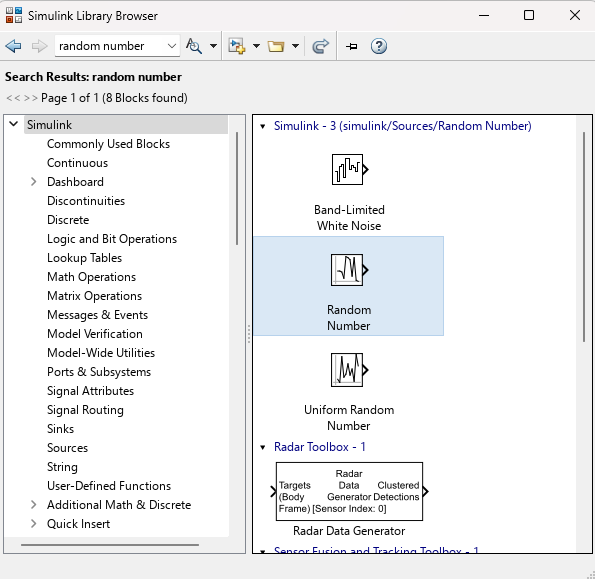
\includegraphics[width=\textwidth]{fig/Capitulo5/Caso_de_estudio_IMU/Generador_de_archivos/libreria_de_bloques_aceleracion_lineal.png}
        \caption{Librería de bloques - Aceleración Lineal}
        \label{fig:lib_bloques_linear_acceleration}
    \end{subfigure}
    \hfill
    \begin{subfigure}[b]{0.45\textwidth}
        \centering
        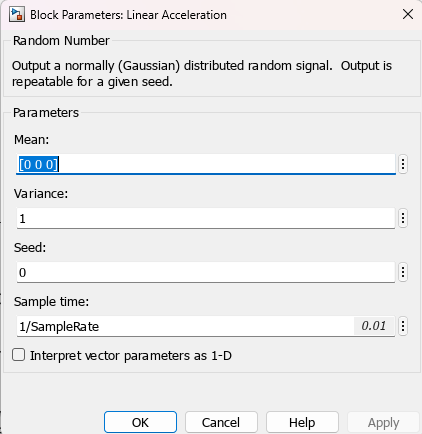
\includegraphics[width=\textwidth]{fig/Capitulo5/Caso_de_estudio_IMU/Generador_de_archivos/configuracion_bloque_aceleracion_lineal.png}
        \caption{Configuración del bloque aceleración lineal}
        \label{fig:lib_bloques_config_linear_acceleration}
    \end{subfigure}
    \caption{Bloque para la aceleración lineal}
    \label{fig:linear_accel_block_simulink}
\end{figure}


\begin{figure}[htbp]
    \centering
    \begin{subfigure}[b]{0.45\textwidth}
        \centering
        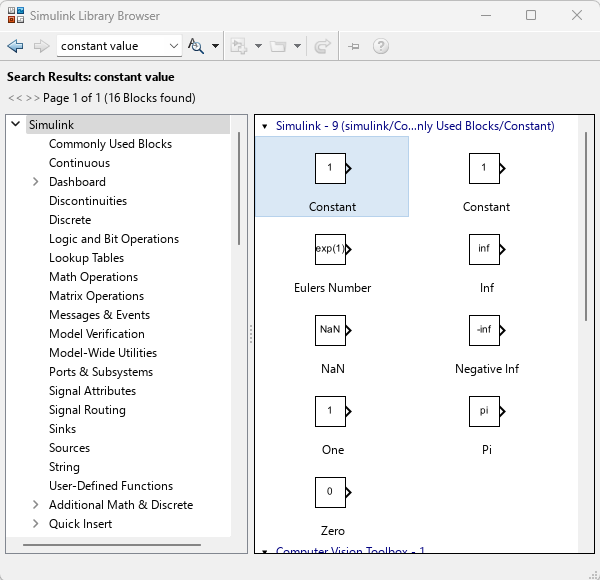
\includegraphics[width=\textwidth]{fig/Capitulo5/Caso_de_estudio_IMU/Generador_de_archivos/libreria_de_bloques_constante_velocidad_angular.png}
        \caption{Librería de bloques - Velocidad Angular}
        \label{fig:lib_bloques_angular_velocity}
    \end{subfigure}
    \hfill
    \begin{subfigure}[b]{0.45\textwidth}
        \centering
        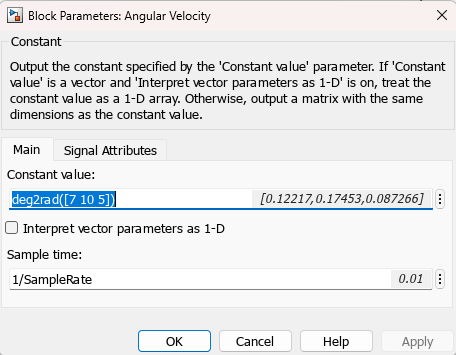
\includegraphics[width=\textwidth]{fig/Capitulo5/Caso_de_estudio_IMU/Generador_de_archivos/configuracion_bloque_velocidad_angular.png}
        \caption{Configuración del bloque velocidad angular}
        \label{fig:lib_bloques_config_angular_velocity}
    \end{subfigure}
    \caption{Bloque para la velocidad angular}
    \label{fig:angular_velocity_block_simulink}
\end{figure}


\begin{figure}[htbp]
    \centering
    % Primera imagen
    \begin{subfigure}[b]{0.35\textwidth}
        \centering
        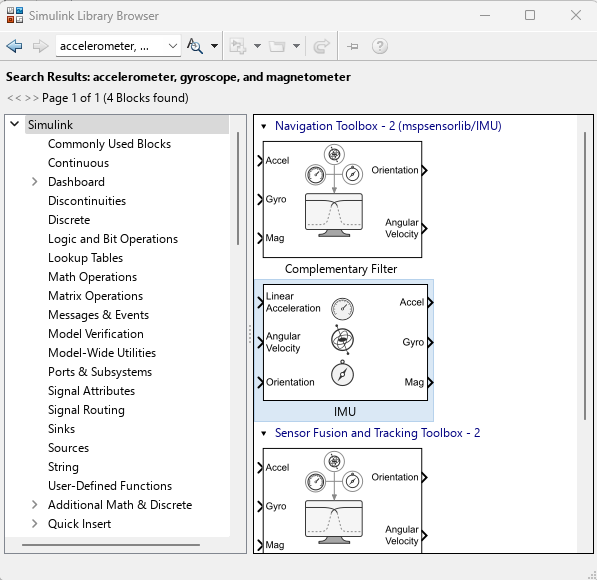
\includegraphics[width=\textwidth]{fig/Capitulo5/Caso_de_estudio_IMU/Generador_de_archivos/libreria_de_bloques_IMU.png}
        \caption{Librería de bloques - IMU}
        \label{fig:lib_bloques_IMU}
    \end{subfigure}
    \hfill
    % Segunda imagen
    \begin{subfigure}[b]{0.45\textwidth}
        \centering
        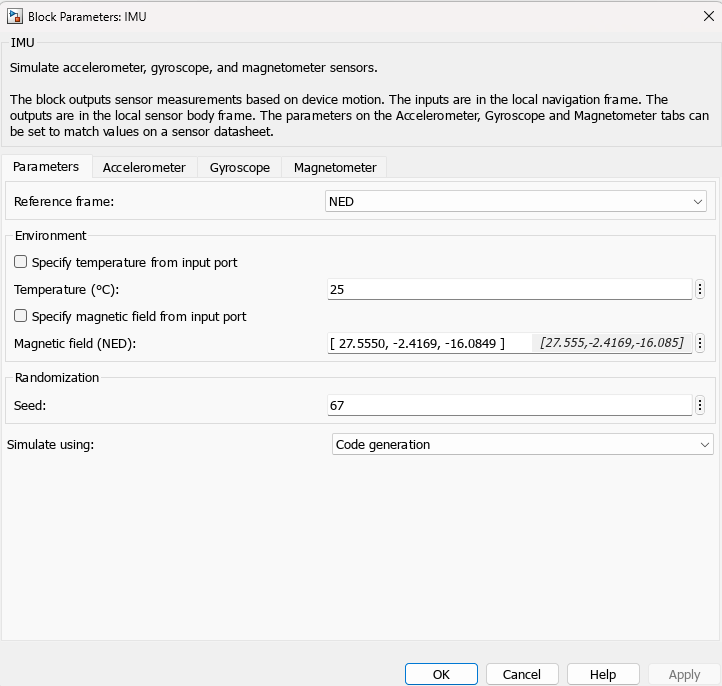
\includegraphics[width=\textwidth]{fig/Capitulo5/Caso_de_estudio_IMU/Generador_de_archivos/configuracion_parametros_IMU_01.png}
        \caption{Configuración de parámetros 1}
        \label{fig:parametros_IMU_01}
    \end{subfigure}
    \hfill
    % Tercera imagen
    \begin{subfigure}[b]{0.45\textwidth}
        \centering
        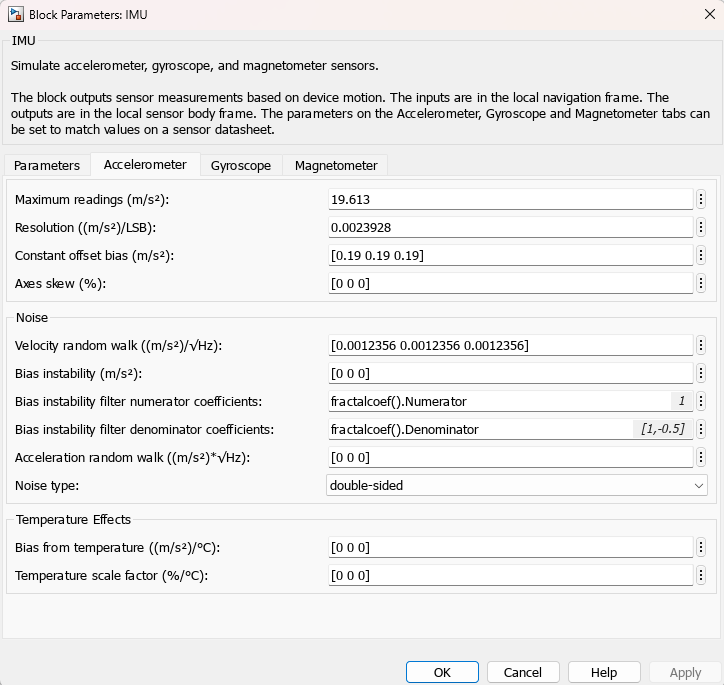
\includegraphics[width=\textwidth]{fig/Capitulo5/Caso_de_estudio_IMU/Generador_de_archivos/configuracion_parametros_IMU_02.png}
        \caption{Configuración de parámetros 2}
        \label{fig:parametros_IMU_02}
    \end{subfigure}
    \hfill
    % Cuarta imagen
    \begin{subfigure}[b]{0.45\textwidth}
        \centering
        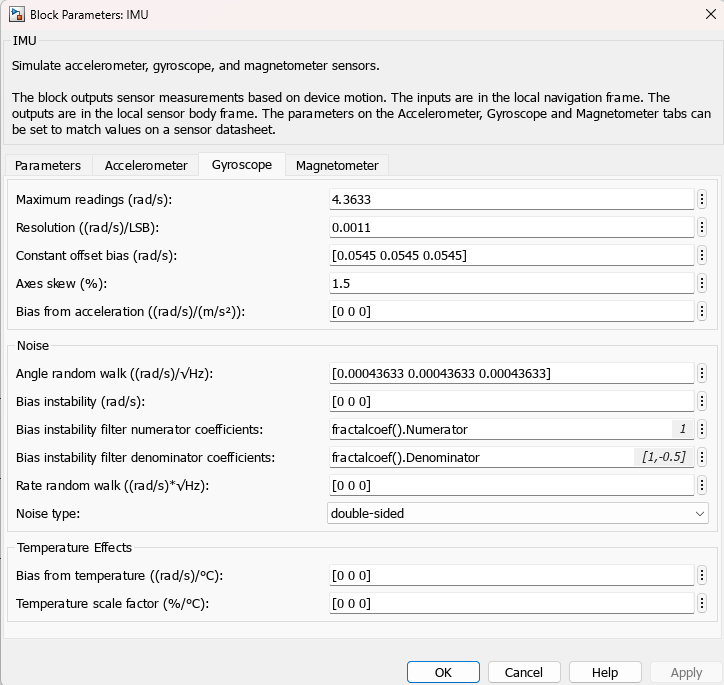
\includegraphics[width=\textwidth]{fig/Capitulo5/Caso_de_estudio_IMU/Generador_de_archivos/configuracion_parametros_IMU_03.png}
        \caption{Configuración de parámetros 3}
        \label{fig:parametros_IMU_03}
    \end{subfigure}
    \hfill
    % Quinta imagen
    \begin{subfigure}[b]{0.45\textwidth}
        \centering
        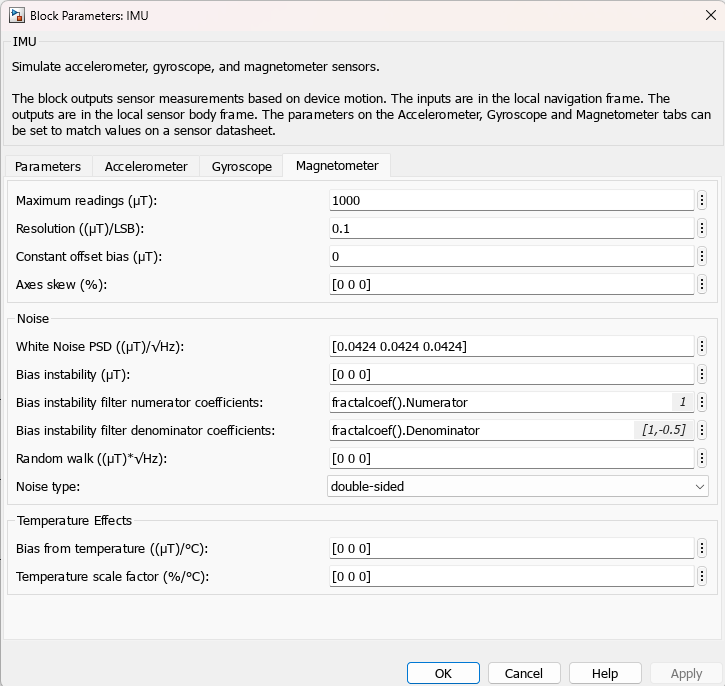
\includegraphics[width=\textwidth]{fig/Capitulo5/Caso_de_estudio_IMU/Generador_de_archivos/configuracion_parametros_IMU_04.png}
        \caption{Configuración de parámetros 4}
        \label{fig:parametros_IMU_04}
    \end{subfigure}

    \caption{Bloque para la simulación del comportamiento de la IMU}
    \label{fig:arreglo_imu}
\end{figure}


\begin{figure}[htbp]
    \centering
    \begin{subfigure}[b]{0.35\textwidth}
        \centering
        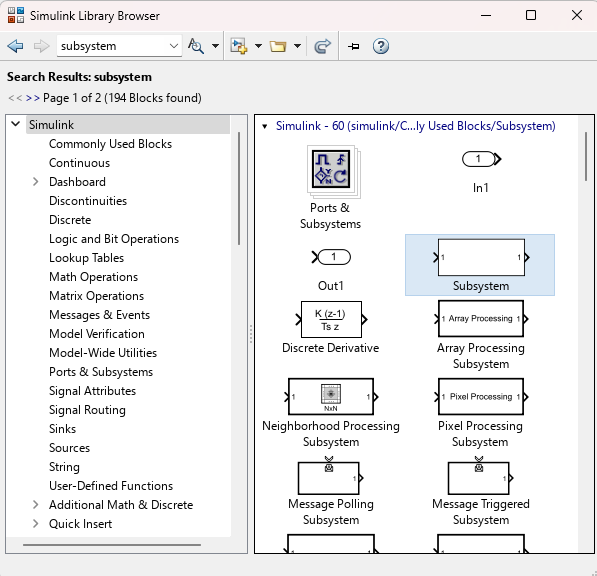
\includegraphics[width=\textwidth]{fig/Capitulo5/Caso_de_estudio_IMU/Generador_de_archivos/libreria_de_bloques_subsistema_integracion_velocidad_angular.png}
        \caption{Librería de bloques - Integrador}
        \label{fig:lib_bloques_integrador}
    \end{subfigure}
    \hfill
    \begin{subfigure}[b]{0.45\textwidth}
        \centering
        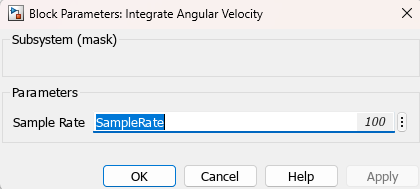
\includegraphics[width=\textwidth]{fig/Capitulo5/Caso_de_estudio_IMU/Generador_de_archivos/configuracion_integrador_velocidad_angular.png}
        \caption{Configuración del bloque velocidad angular}
        \label{fig:config_bloques_integrador}
    \end{subfigure}
    \caption{Bloque para la integración de la velocidad angular}
    \label{fig:integration_for_angular_velocity}
\end{figure}


%Missing image for required block information
%\begin{figure}[htbp]
%    \centering
%    \begin{subfigure}[b]{0.35\textwidth}
%        \centering
%        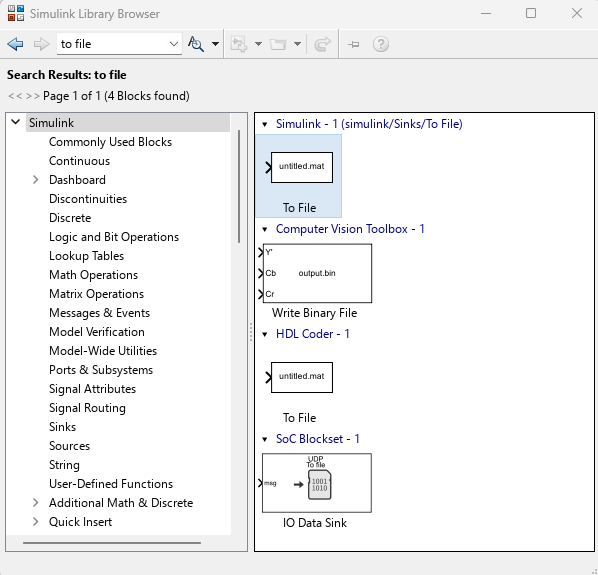
\includegraphics[width=\textwidth]{fig/Capitulo5/Caso_de_estudio_IMU/Generador_de_archivos/libreria_de_bloques_to_file.png}
%        \caption{Librería de bloques - Guardar en archivo}
%        \label{fig:lib_bloques_to_file_IMU}
%    \end{subfigure}
%    \hfill
%    \begin{subfigure}[b]{0.45\textwidth}
%        \centering
%        \includegraphics[width=\textwidth]{fig/Capitulo5/Caso_de_estudio_IMU/Generador_de_archivos/}
%        \caption{}
%        \label{fig:}
%    \end{subfigure}
%    \caption{}
%    \label{fig:}
%\end{figure}


\subsubsection{Sistema para la lectura e interpretación de los archivos generados previamente}

\begin{figure}[htbp]
    \centering
    \begin{subfigure}[b]{0.35\textwidth}
        \centering
        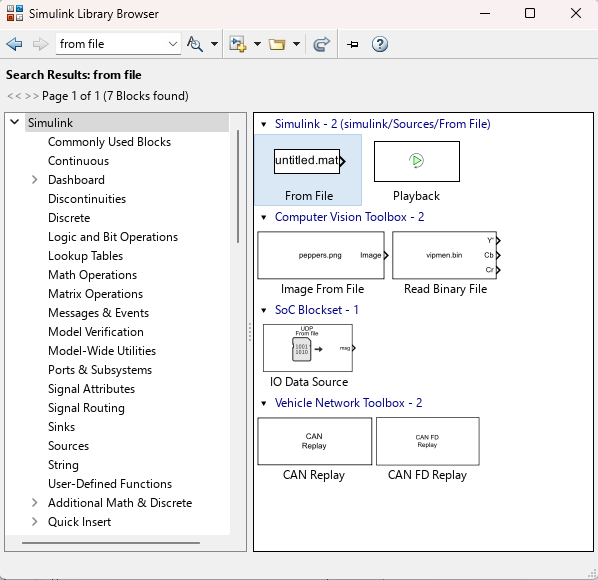
\includegraphics[width=\textwidth]{fig/Capitulo5/Caso_de_estudio_IMU/Generador_de_salidas/libreia_de_bloques_from_file.png}
        \caption{Librería de bloques - Leer de archivo}
        \label{fig:lib_bloques_from_file_IMU}
    \end{subfigure}
    \hfill
    \begin{subfigure}[b]{0.45\textwidth}
        \centering
        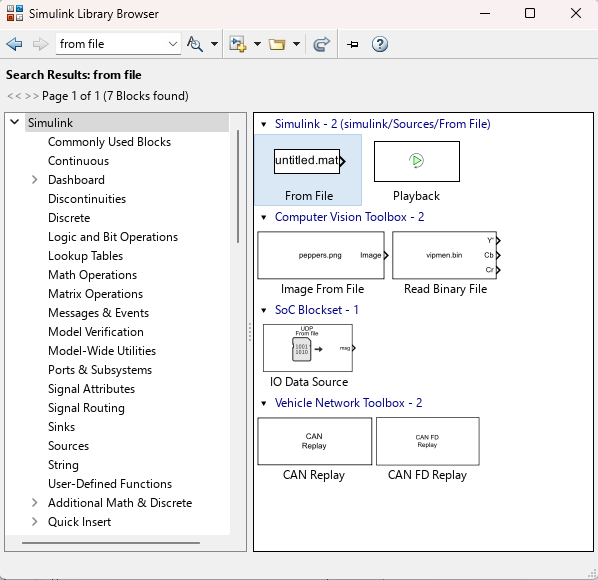
\includegraphics[width=\textwidth]{fig/Capitulo5/Caso_de_estudio_IMU/Generador_de_salidas/libreia_de_bloques_from_file.png}
        \caption{Configuración del bloque encargado de la lectura de archivos}
        \label{fig:config_from_file_IMU}
    \end{subfigure}
    \caption{Bloque para la lectura de archivos}
    \label{fig:read_from_file}
\end{figure}


\begin{figure}[htbp]
    \centering
    \begin{subfigure}[b]{0.35\textwidth}
        \centering
        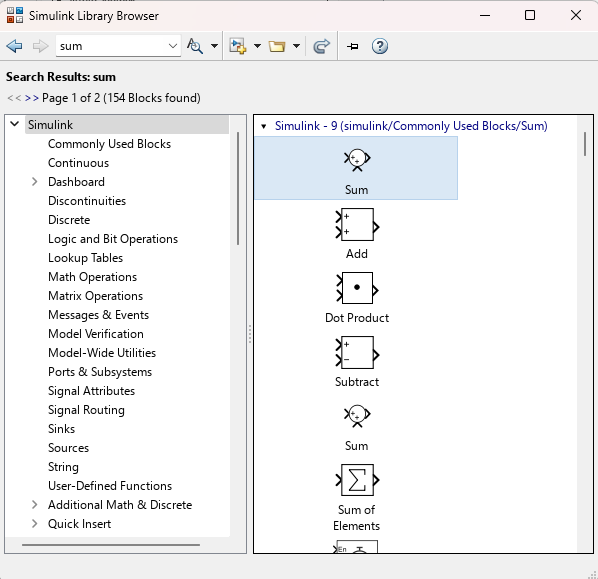
\includegraphics[width=\textwidth]{fig/Capitulo5/Caso_de_estudio_IMU/Generador_de_salidas/libreia_de_bloques_suma.png}
        \caption{Librería de bloques - Suma}
        \label{fig:lib_bloques_add_IMU}
    \end{subfigure}
    \hfill
    \begin{subfigure}[b]{0.45\textwidth}
        \centering
        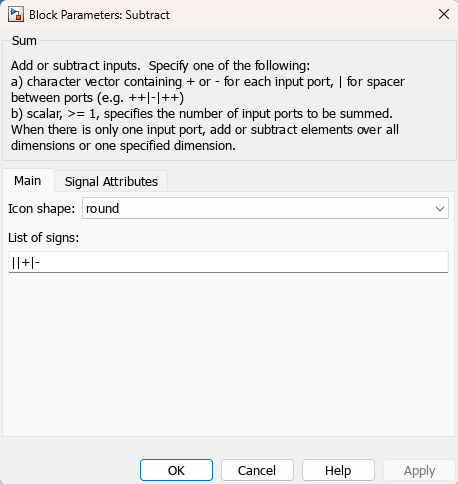
\includegraphics[width=\textwidth]{fig/Capitulo5/Caso_de_estudio_IMU/Generador_de_salidas/configuracion_bloque_suma.png}
        \caption{Configuración del bloque encargado de la suma de señales}
        \label{fig:config_add_IMU}
    \end{subfigure}
    \caption{Bloque para la suma de señales}
    \label{fig:add_of_some_signals}
\end{figure}


\begin{figure}[htbp]
    \centering
    % Primera imagen
    \begin{subfigure}[b]{0.35\textwidth}
        \centering
        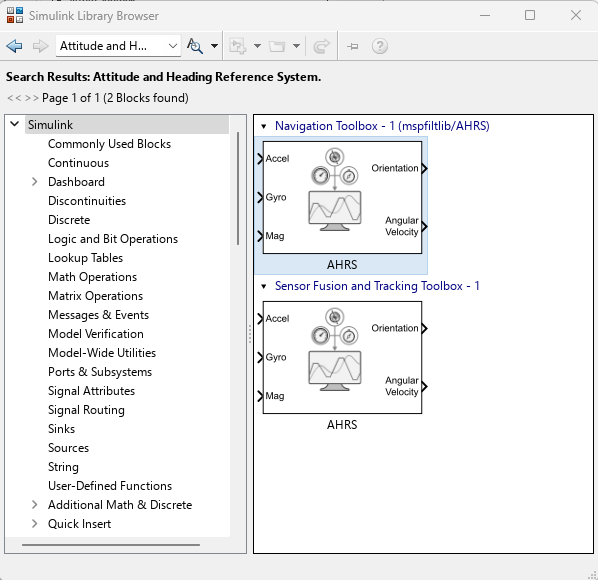
\includegraphics[width=\textwidth]{fig/Capitulo5/Caso_de_estudio_IMU/Generador_de_salidas/libreira_de_bloques_sensor_AHRS.png}
        \caption{Librería de bloques - AHRS}
        \label{fig:lib_bloques_AHRS}
    \end{subfigure}
    \hfill
    % Segunda imagen
    \begin{subfigure}[b]{0.45\textwidth}
        \centering
        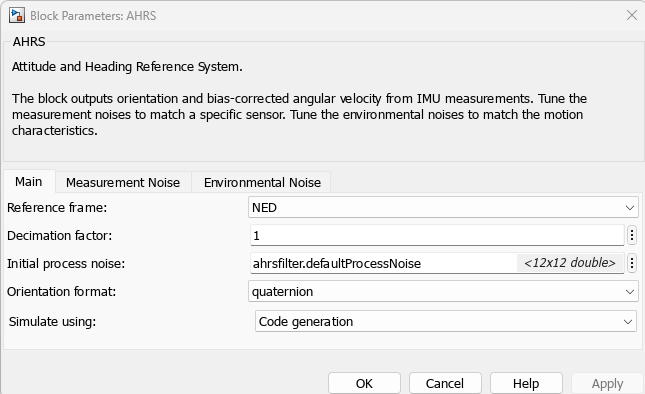
\includegraphics[width=\textwidth]{fig/Capitulo5/Caso_de_estudio_IMU/Generador_de_salidas/configuracion_AHRS_01.png}
        \caption{Configuración de parámetros 1}
        \label{fig:parametros_AHRS_01}
    \end{subfigure}
    \hfill
    % Tercera imagen
    \begin{subfigure}[b]{0.45\textwidth}
        \centering
        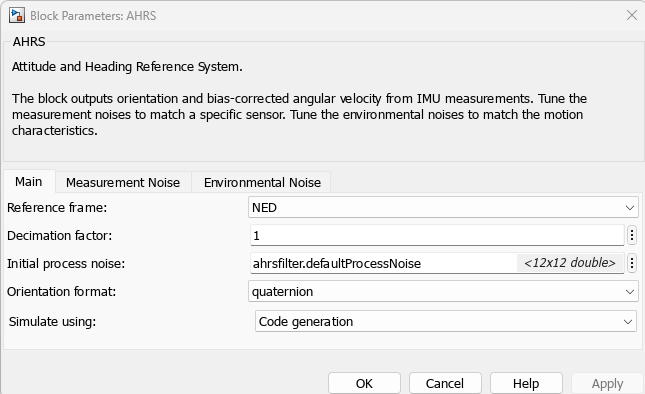
\includegraphics[width=\textwidth]{fig/Capitulo5/Caso_de_estudio_IMU/Generador_de_salidas/configuracion_AHRS_01.png}
        \caption{Configuración de parámetros 2}
        \label{fig:parametros_AHRS_02}
    \end{subfigure}
    \hfill
    % Cuarta imagen
    \begin{subfigure}[b]{0.45\textwidth}
        \centering
        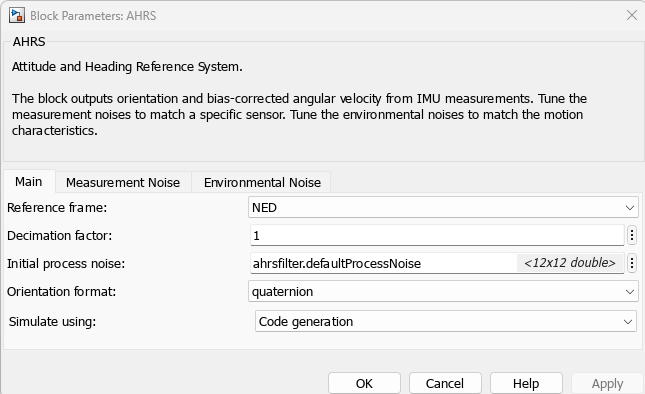
\includegraphics[width=\textwidth]{fig/Capitulo5/Caso_de_estudio_IMU/Generador_de_salidas/configuracion_AHRS_01.png}
        \caption{Configuración de parámetros 3}
        \label{fig:parametros_AHRS_03}
    \end{subfigure}

    \caption{Bloque para la simulación del comportamiento de la IMU}
    \label{fig:arreglo_AHRS}
\end{figure}

\begin{figure}[htbp]
    \centering
    \begin{subfigure}[b]{0.35\textwidth}
        \centering
        \includegraphics[width=\textwidth]{fig/Capitulo5/Caso_de_estudio_IMU/Generador_de_salidas/libreria_bloque__rad_2_deg.png}
        \caption{Librería de bloques - Conversor de radianes a grados}
        \label{fig:lib_bloques_R2D}
    \end{subfigure}
    \hfill
    \begin{subfigure}[b]{0.45\textwidth}
        \centering
        \includegraphics[width=\textwidth]{fig/Capitulo5/Caso_de_estudio_IMU//Generador_de_salidas/libreria_bloque__rad_2_deg.png}
        \caption{Configuración del bloque conversor de radianes a grados}
        \label{fig:conf_bloques_R2D}
    \end{subfigure}
    \caption{Bloque para convertir de Radianes a grados}
    \label{fig:bloques_R2D}
\end{figure}


\begin{figure}[htbp]
    \centering
    \begin{subfigure}[b]{0.35\textwidth}
        \centering
        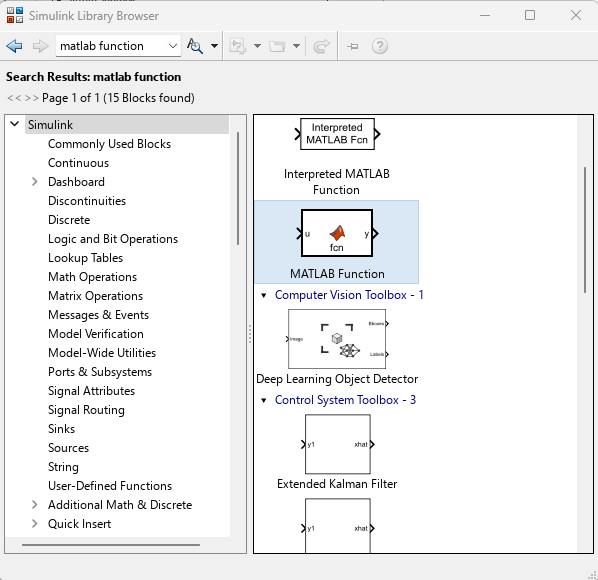
\includegraphics[width=\textwidth]{fig/Capitulo5/Caso_de_estudio_IMU/Generador_de_salidas/libreria_bloque_de_funcion.png}
        \caption{Librería de bloques - Función}
        \label{fig:lib_bloques_func}
    \end{subfigure}
    \hfill
    \begin{subfigure}[b]{0.45\textwidth}
        \centering
        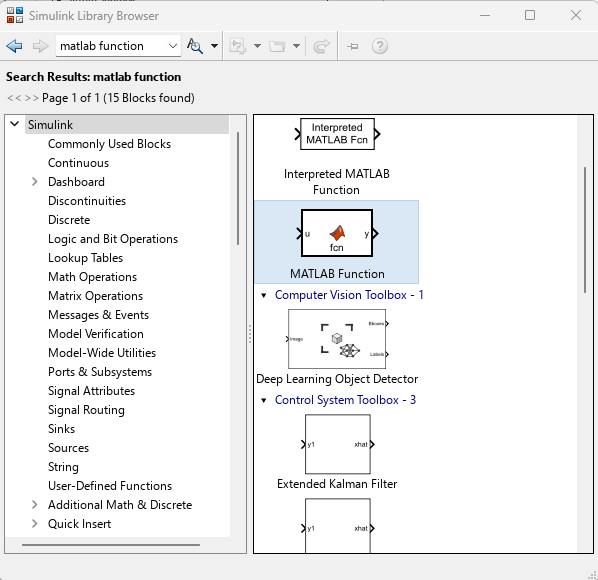
\includegraphics[width=\textwidth]{fig/Capitulo5/Caso_de_estudio_IMU/Generador_de_salidas/libreria_bloque_de_funcion.png}
        \caption{}
        \label{fig:config_bloques_func}
    \end{subfigure}
    \caption{Bloque para aplicar una función implementada mediante código}
    \label{fig:bloques_func}
\end{figure}

\subsection{Resultados de la simulación}

\subsection{Implementación en la Tarjeta de desarrollo mediante EmbedSynthGNC}

Para la implementación en la tarjeta de desarrollo ZedBoard se ejecuta el flujo de trabajo que se muestra en la sección \ref{}. El mismo es representado mediante el diagrama que se muestra en la Figura \ref{}.



\subsection{Resultados de la implementación}

\section{Caso de estudio 3 - PID}

Finalmente como ultimo caso de estudio se desarrolla un controlador PID (Proporcional-Integral-Derivativo) es una herramienta clave en los sistemas de control automático, diseñada para minimizar el error entre una señal de referencia y la señal de salida real. Su importancia radica en su capacidad para ajustar la respuesta del sistema, logrando un equilibrio entre rapidez y estabilidad. Esto permite que el controlador maneje eficazmente perturbaciones y cambios en el entorno, siendo aplicable a una variedad de sistemas, como motores eléctricos, sistemas de calefacción y procesos industriales complejos.

En el contexto de MATLAB y Simulink, estas herramientas ofrecen una plataforma visual que facilita la implementación y ajuste de controladores PID. A través de bloques específicos en Simulink, los ingenieros pueden modificar en tiempo real los parámetros proporcional, integral y derivativo, observando directamente cómo estos ajustes afectan la salida del sistema. Esta capacidad de simulación y diseño iterativo no solo optimiza el rendimiento del sistema controlado, sino que también proporciona un entorno propicio para la experimentación y el aprendizaje práctico en el campo del control automático.


\subsection{Implementación en MATLAB Simulink}

\begin{figure}[h!]
    \centering
    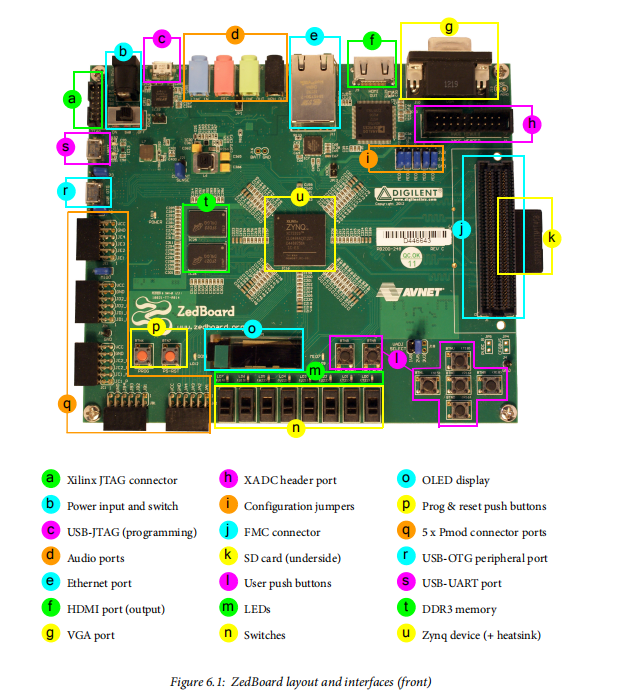
\includegraphics[width=0.8\textwidth]{fig/especifico_2/154140ZedBoard.png}
    \caption{Diagrama completo del caso de estudio 3 - PID }
    \label{fig:caso_de_estudio_3_PID}
\end{figure}


Como se puede observar en la Figura \ref{fig:caso_de_estudio_3_PID}, este es el caso de estudio que se propone en \cite{microcontrollerslab_pid_controller_design}, a este caso de estudio se le deben de realizar unas modificaciones de acuerdo al funcionamiento deseado que se tiene para este caso de estudio, siempre generando datos en el ámbito de simulación en MATLAB para luego contrastar los mismos con los datos obtenidos en la ejecución del modelo en la tarjeta de desarrollo seleccionada.

\subsection{Bloques utilizados para la implementación}

Los bloques utilizados se obtienen en la librería de bloques de MATLAB Simulink. A continuación se muestran los bloques requeridos, asi como la configuración de los mismos para la correcta operación del modelo. La implementación del sistema se divide en dos partes, el primer parte se encarga de generar los archivos necesarios para la operación del sistema mientras que la segunda parte del sistema se encarga de leer los archivos con los datos y generar los dos archivos de salida del programa.

\subsubsection{Sistema para la generación de archivos}

Este sistema es el encargado de generar los archivos de entrada, estos mismos contienen los datos de tiempo y valores para la correcta implementación del sistema

\subsection{Implementación en la Tarjeta de desarrollo mediante EmbedSynthGNC}